%
%     hw3_bbordwell.tex
%     Baylee Bordwell (baylee.bordwell@colorado.edu)
%     Based on the template by Benjamin Brown (bpbrown@colorado.edu)
%     Aug 27, 2014
%
%     Problem set 3 for ASTR/ATOC 5540, Mathematical Methods, taught at
%     University of Colorado, Boulder, Fall 2014.
%
%

\documentclass[12pt, preprint]{aastex}
% formatting based on 2014 NASA ATP proposal with Jeff Oishi

%%%%%%begin preamble
\usepackage[hmargin=1in, vmargin=1in]{geometry} % Margins
\usepackage{hyperref}
\usepackage{url}
\usepackage{times}
\usepackage{natbib}
\usepackage{graphicx}
\usepackage{amsmath}
\usepackage{amsfonts}
\usepackage{amssymb}
\usepackage{pdfpages}
\usepackage{import}
% for code import
\usepackage{listings}
\usepackage{color}
\usepackage{ragged2e}

\hypersetup{
     colorlinks   = true,
     citecolor     = gray,
     urlcolor       = blue
}

%% headers
\usepackage{fancyhdr}
\pagestyle{fancy}
\lhead{ASTR/ATOC 5540}
\chead{}
\rhead{name: Baylee Bordwell}
\lfoot{Problem Set 3}
\cfoot{\thepage}
\rfoot{Fall 2014}
% no hline under header
\renewcommand{\headrulewidth}{0pt}

\newcommand{\sol}{\ensuremath{\odot}}

% make lists compact
\usepackage{enumitem}
%\setlist{nosep}

%%%%%%end preamble


\begin{document}
\section*{Problem Set 3: Fitting Solar/Stellar data without error}
\begin{enumerate}
\item 
\begin{figure}[!ht]  \centering
  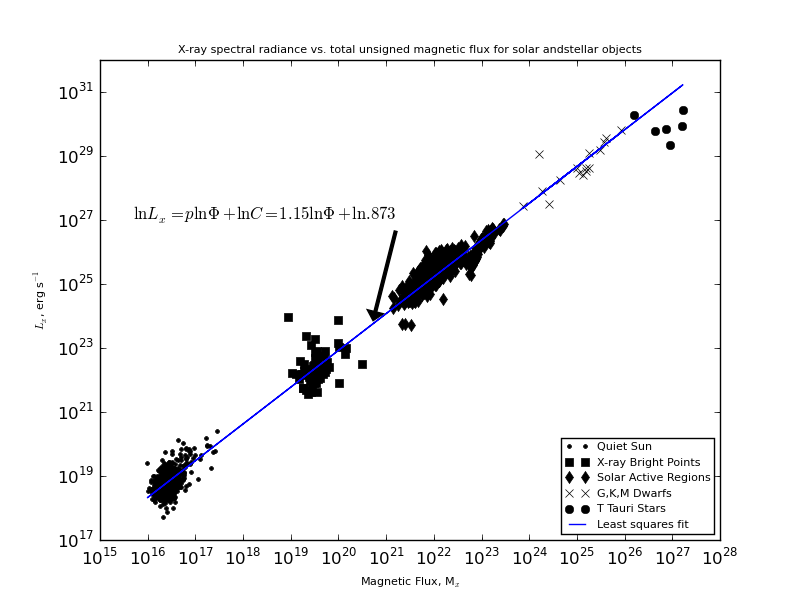
\includegraphics[width=5in]{hw3_fig.png}
\end{figure}

\item $L_x = C * \Phi^p$ $\Rightarrow$ $\ln(L_x) = p\ln(\Phi) + \ln(C)$ \newline
For $n$ unknowns, the system of equations, $A\mathbf{x} = \mathbf{b}$ holds, where for an unknown n $\mathbf{b_n}$ is $L_{x,n}$, $x_1$ is $p$, $x_2$ is $\ln(C)$, $A_{n1}$ is $\ln{\Phi}$ and $A_{n2}$ is 1.

\item The \verb|mflux_lx_all.txt| file is 1316 lines long, so $n = 1316$. $A$ is 2 by $n$, $\mathbf{x}$ is 1 by 2, and $\mathbf{b}$ is 1 by $n$. The system of equations looks like,
\[\left(\begin{array}{cc}
$A_{11}$ & $A_{12}$ \\
$A_{21}$ & $A_{22}$ \\
\vdots & \vdots \\
$A_{n1}$ & $A_{n2}$ \\
\end{array}\right)
\left(\begin{array}{c}
$x_1$ \\
$x_2$ \\
\end{array}\right) = 
\left( \begin{array}{c}
$b_1$ \\
$b_2$ \\
\vdots \\
$b_n$ \\
\end{array}\right)
\]

\item 
\[ \begin{array}{l}
$A\mathbf{x}=\mathbf{b}$ \\
$A^TA\mathbf{x}=A^T\mathbf{b}$ \\
$\mathbf{x}=(A^TA)^{-1}A^T\mathbf{b}$ \\
\end{array}
\] 
The value of $\mathbf{x}$ found above minimizes $(A\mathbf{x}-\mathbf{b})^T(A\mathbf{x}-\mathbf{b})$ because it is the solution to the equation $(A\mathbf{x}-\mathbf{b})=0$ and  $(A\mathbf{x}-\mathbf{b})^T(A\mathbf{x}-\mathbf{b})$ is effectively  ``$(A\mathbf{x}-\mathbf{b})^2$'', so with $\mathbf{x}$ as above $(A\mathbf{x}-\mathbf{b})^T(A\mathbf{x}-\mathbf{b})=0$, which is the minimum value for a real squared number.

\item Solving for x yields: $p = 1.1492$, $C = 8.7255\cdot 10^{-1}$ \newline
My $p$ does agree with Pevtsov et al. (2003).

\item Overplotted in the figure in question 1. The mean absolute error in logspace of the fit is $1.99\cdot 10^{-2}$. If the mean absolute error was calculated in non-logspace, it would be huge, because the linear fit optimizes the fit to have approximately the same error for all points, and the scale of the error for the points with higher M$_x$ would suddenly be much greater than that of points with lower M$_x$.
\end{enumerate}

\noindent Code involved in this assignment:
%
%     hw2_code.tex
%     Benjamin Brown (bpbrown@colorado.edu)
%     Aug 27, 2014
%
%     Problemset 2 for ASTR/ATOC 5540, Mathematical Methods, taught at
%     University of Colorado, Boulder, Fall 2014.
%
%     Python code importing block.
%


\definecolor{codegreen}{rgb}{0,0.6,0}
\definecolor{codegray}{rgb}{0.5,0.5,0.5}
\definecolor{codepurple}{rgb}{0.58,0,0.82}
\definecolor{backcolour}{rgb}{0.95,0.95,0.92}
 
\lstdefinestyle{mystyle}{
    backgroundcolor=\color{backcolour},   
    commentstyle=\color{codegreen},
    keywordstyle=\color{magenta},
    numberstyle=\tiny\color{codegray},
    stringstyle=\color{codepurple},
    basicstyle=\footnotesize,
    breakatwhitespace=false,         
    breaklines=true,                 
    captionpos=b,                    
    keepspaces=true,                 
    numbers=left,                    
    numbersep=5pt,                  
    showspaces=false,                
    showstringspaces=false,
    showtabs=false,                  
    tabsize=2
}

\lstset{style=mystyle}


\lstinputlisting[language=Python]{hw3_bbordwell.py}


\end{document}
